% Dipolar magnetic field
% Author: Cyril Langlois
%
% A 3D plot of a dipolar magnetic field similar to the Earth's one.
% The field lines are drawn in each longitude plane using the dipolar field
% equation. Like Earth's field, the north magnetic pole lies close to the south
% geographic pole and vice-versa.
%
% The code is based on the Tomasz M. Trzeciak code for stereographic drawing and the plot command.
\documentclass[11pt]{article}
\usepackage{tikz}
\usetikzlibrary{arrows,calc}
%%% Macro's for 3D figures %%%
\newcommand\pgfmathsinandcos[3]{%
    \pgfmathsetmacro#1{sin(#3)}%
    \pgfmathsetmacro#2{cos(#3)}%
}
\newcommand\LongitudePlane[3][current plane]{%
    \pgfmathsinandcos\sinEl\cosEl{#2} % elevation
    \pgfmathsinandcos\sint\cost{#3}   % azimuth
    \tikzset{#1/.estyle={cm={\cost,\sint*\sinEl,0,\cosEl,(0,0)}}}
}
\newcommand\LatitudePlane[3][current plane]{%
    \pgfmathsinandcos\sinEl\cosEl{#2} % elevation
    \pgfmathsinandcos\sint\cost{#3}   % latitude
    \pgfmathsetmacro\yshift{\cosEl*\sint}
    \tikzset{#1/.estyle={cm={\cost,0,0,\cost*\sinEl,(0,\yshift)}}} %
}
\newcommand\DrawLongitudeCircle[2][1]{
    \LongitudePlane{\angEl}{#2}
    \tikzset{current plane/.prefix style={scale=#1}}
    % angle of "visibility"
    \pgfmathsetmacro\angVis{atan(sin(#2)*cos(\angEl)/sin(\angEl))} %
    \draw[current plane] (\angVis:1) arc (\angVis:\angVis+180:1);
    \draw[current plane,dashed] (\angVis-180:1) arc (\angVis-180:\angVis:1);
}
\newcommand\DrawLatitudeCircle[2][1]{
    \LatitudePlane{\angEl}{#2}
    \tikzset{current plane/.prefix style={scale=#1}}
    \pgfmathsetmacro\sinVis{sin(#2)/cos(#2)*sin(\angEl)/cos(\angEl)}
    % angle of "visibility"
    \pgfmathsetmacro\angVis{asin(min(1,max(\sinVis,-1)))}
    \draw[current plane] (\angVis:1) arc (\angVis:-\angVis-180:1);
    \draw[current plane,dashed] (180-\angVis:1) arc (180-\angVis:\angVis:1);
}


\begin{document}
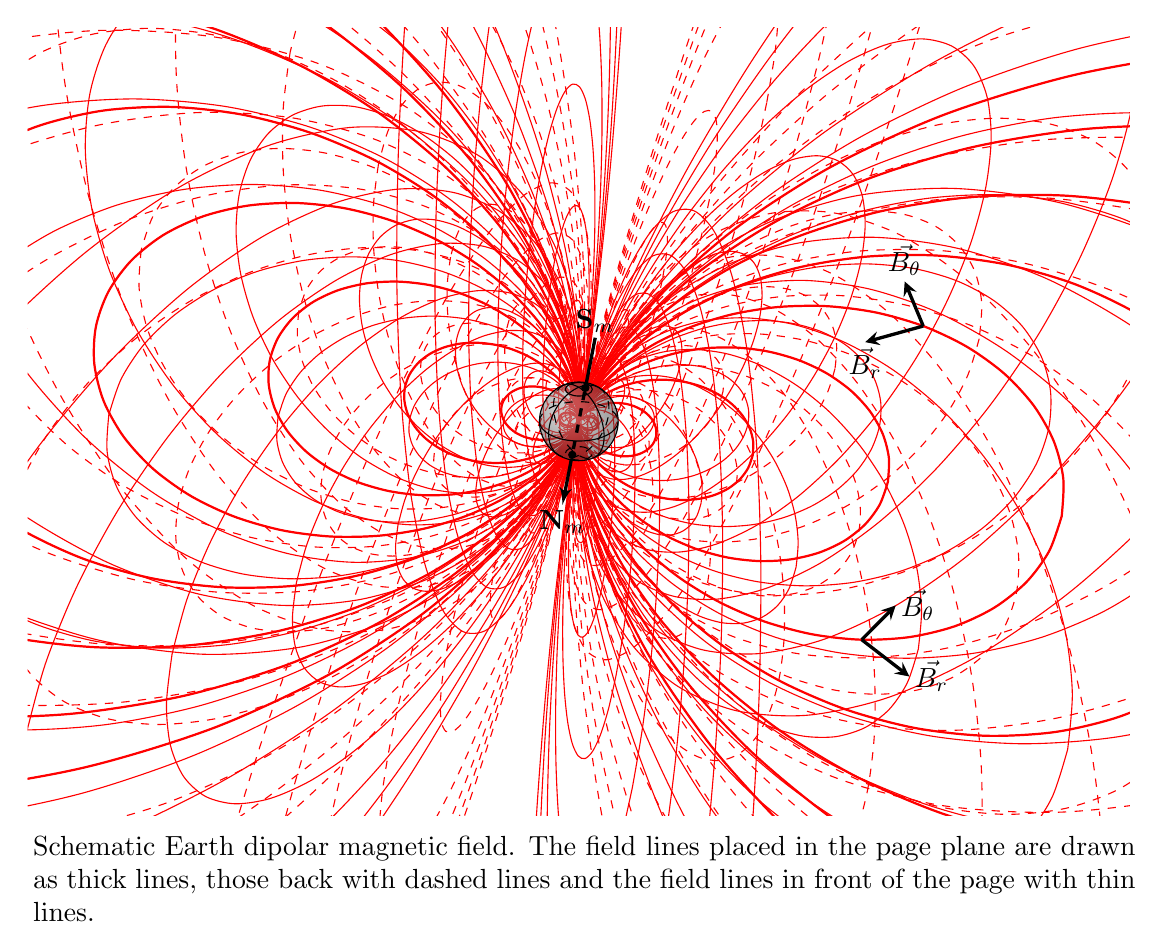
\begin{tikzpicture}[scale=1.0,
        %Option for nice arrows%
        >=latex,%
        inner sep=0pt,%
        outer sep=2pt,%
        mark coordinate/.style={outer sep=0pt,
            minimum size=3pt, fill=black,circle}%
    ]
    %% some definitions
    \def\R{0.5}       % sphere radius
    \def\angEl{30}    % elevation angle
    \def\angAz{-140}  % azimuth angle
    \def\angPhi{-105} % longitude of point
    \def\angBeta{55}  % latitude of point
    \def\angGam{-190} % longitude of point
    %% working planes
    \pgfmathsetmacro\H{\R*cos(\angEl)}          % Distance to north pole
    \LongitudePlane[xzplane]{\angEl}{\angAz}    % x-axis plane
    %
    \coordinate (O) at (0,0);
    %
    \begin{scope}[rotate around={-11.1:(0,0)},
        field line/.style={color=red, smooth,
            variable=\t, samples at={0,-5,-10,...,-360}}
    ]
        \clip[rotate around={11.1:(0,0)}] (-7,5) rectangle (7,-5);

        % Computes a point on a field line given r and t
        \newcommand{\fieldlinecurve}[2]{%
            {(pow(#1,2))*(3*cos(#2)+cos(3*#2))}, {(pow(#1,2))*(sin(#2)+sin(3*#2))}%
        }

        % Longitudinal plnaes
        \foreach \u in {0,-40,...,-160}{
            \LongitudePlane[{{\u}zplane}]{\angEl}{\u}
            \foreach \r in {0.25,0.5,...,2.25} {
                \draw[{{\u}zplane}, field line]
                plot (\fieldlinecurve{\r}{\t});
            }
        }
        \foreach \u in {-200,-240,...,-320}{
            \LongitudePlane[{{\u}zplane}]{\angEl}{\u}
            \foreach \r in {0.25,0.5,...,2.25}{
            \draw[{{\u}zplane}, dashed, field line]
                plot (\fieldlinecurve{\r}{\t});
            }
        }
        % Drawing plane for the B-vectors
        \LongitudePlane[bzplane]{\angEl}{0}
            \foreach \r in {0.25,0.5,...,2.25}{
            \draw[bzplane, thick, field line]
                plot (\fieldlinecurve{\r}{\t});
        }

        \begin{scope}[bzplane, very thick, ->, >=stealth]
            \draw (\fieldlinecurve{1.25}{-30}) -- +(-30:0.79cm)  node[right] {$\vec{B_{r}}$};
            \draw (\fieldlinecurve{1.25}{-30}) -- +(60:0.68cm)   node[right] {$\vec{B_{\theta}}$};
            \draw (\fieldlinecurve{1.25}{30})  -- +(-150:0.79cm) node[below] {$\vec{B_{r}}$};
            \draw (\fieldlinecurve{1.25}{30})  -- +(120:0.68cm)  node[above] {$\vec{B_{\theta}}$};
        \end{scope}
        %
        \begin{scope}[rotate around={11.1:(0,0)}]
            \fill[ball color=white,opacity=0.3] (O) circle (\R); %3D lighting effect
            \draw (O) circle (\R);
            \DrawLongitudeCircle[\R]{\angAz}      % xzplane
            \DrawLongitudeCircle[\R]{\angAz + 90} % vzplane
            \DrawLatitudeCircle[\R]{0}            % equator
            \DrawLatitudeCircle[\R]{70}           % Latitude 70
            \DrawLatitudeCircle[\R]{-70}          % Latitude -70
        \end{scope}
        %
        \coordinate[mark coordinate] (Sm) at (0, \H);
        \coordinate[mark coordinate] (Nm) at (0,-\H);
        \path[xzplane] (Nm) -- +(0,-0.75) coordinate (Nm1) node[below] {$\mathbf{N}_m$}
                       (Sm) -- +(0,0.75)  coordinate (Sm1) node[above] {$\mathbf{S}_m$};
        \draw[very thick, dashed]    (Sm) -- (Nm);
        \draw[very thick]            (Sm1) -- (Sm);
        \draw[very thick,->,>=latex'](Nm) -- (Nm1);
    \end{scope}
    \node[align=justify, text width=14cm, anchor=north west] at (-7,-5.2)
        {Schematic Earth dipolar magnetic field. The field lines placed in the
        page plane are drawn as thick lines, those back with dashed lines and
        the field lines in front of the page with thin lines.};
\end{tikzpicture}
\end{document}